

\documentclass[12pt, a4paper]{article}
\usepackage[table]{xcolor}
\usepackage[utf8]{inputenc}
\usepackage{multirow}
\usepackage{longtable}
\usepackage{subfig}
\usepackage{graphicx}
\usepackage{eurosym}
\usepackage{pagecolor}
\usepackage{adjustbox}
\usepackage{float}


\pagecolor{white}



\title{STA101 - FOAD : Analyse des données}
\author{Jhon Steven Neira}
\date{February 2022}

  
\begin{document}
  
\maketitle
  
\tableofcontents

\section{Récolte des  données }
% !TEX root = collect.tex

Les données ont été collectées a travers d'un script que trace le comportement d'un utilisateur sur le site web puis sont stockés dans une base de données à des fins de marketing et de tests statistiques, comme collaborateur de cette entreprise et avec son consentement, j'ai exécuté des requêtes dans las base de données pour obtenir ce jeu de données que contient des variables que je considère comme les plus significatives pour examiner le comportement d'achat des utilisateurs.



\section{Objectif}
% !TEX root = Objectif.tex
Comprendre les différents comportements d'un client est souvent un défi. Les méthodes d'analyse  de données sont un moyen essentiel pour nous aider à trouver des réponses qui nous permettront  d'analyser ces comportements. 
Cette étude vise à analyser les transactions sur un site d'e-commerce, nous appliquerons ces  techniques pour décrire un ensemble de données qui contient 1000 sessions d'utilisateurs qui ont  effectué au moins une transaction sur ce site d'e-commerce.  
Quelles sont les transactions similaires et celles qui sont totalement différentes ? Et comment varient-elles en fonction des dispositifs et outils utilisé par l'utilisateur pour effectuer les  transactions.






\section{Étude préliminaire}
% !TEX root = preliminaryStudy.tex

\subsection{Nettoyage des données}
Nous disposons de 1000 sessions d'individus qui ont effectué au moins une transaction, nous avons trouvé quelques individus qui apparaissent deux fois dans l'échantillon et nous voudrions composer les données avec des individus différents pour éviter de polluer  les données.

\subsection{Description des données}
Ci-dessous se trouve une description de chacune des variables de l'ensemble de données, à l'exception de la variable \textit{fullVisitorId} lequelle est un hash composé de 16 caractères alphanumériques pour identifier le visiteur.



\begin{center}
\begin{longtable}{ |p{3cm}||p{3cm}|p{2cm}|p{5cm}|  }
 \hline
 \multicolumn{4}{|c|}{Variables} \\
 \hline
 Nom & Type &Intervalle&Définition\\
 \hline
 hits   & Quantitative discrète  &[9,800]&  Les hits sont les interactions des utilisateurs sur le site web.\\
New visit &   Binaire   & [0, 1]   & C'est la première visite sur le site.\\
Page views&   Quantitative discrète  & [1, 137]   &Est une page chargée (ou rechargée) dans un navigateur.\\
Total transaction revenue & Quantitative continue  &[8.950, 871.380]&  Le revenu associé à la transaction. Cette valeur peut inclure les frais d'expédition, les taxes ou d'autres ajustements du revenu.\\
Transactions    &Quantitative discrète  & [1, 6] &  Nombre de transactions du client dans la session.\\
Time on site&   Quantitative continue  & [68, 8558]& Temps sur le site avant d'effectuer la transaction \\
 Browser name& Qualitative nominal  & -   & Nom du navigateur web.\\
 Browser width& Quantitative continue  & [320, 2560]& La largeur de la fenêtre du navigateur \\
 Browser height& Quantitative continue  & [280, 1356]& La hauteur de la fenêtre du navigateur\\
 Device category& Qualitative nominal   & -&Le dispositif par lequel l'utilisateur a effectué la transaction.\\
 Operating system& Qualitative nominal  & -&Le système d'exploitation par lequel l'utilisateur a effectué la transaction\\
 Language& Qualitative nominal  & -& La langue du navigateur au moment de la transaction.\\
 Country& Qualitative nominal   & -& Le pays depuis où l'utilisateur a effectué la transaction.\\
 Payment method& Qualitative nominal   & -&  Représente  ce que l'utilisateur a utilisé pour payer la transaction.\\
 Item count& Quantitative discrète  & [1, 18]& Un item représente un produit individuel acheté dans le cadre de la transaction. \\
 \hline
\end{longtable}
\end{center}

\subsection{Description des variables}
UnivariePour commencer, ce rapport comportera une analyse univariée de chacune des variables quantitatives et qualitatives qui font partie de le jeu de données, en suite il passera a l'analyse bivariée pour vérifier des liens entre les variables quantitatives mesurées par la corrélation linéaire.







\section{Analyse univariée}
% !TEX root = univariate.tex
\begin{table}[!htbp] \centering 
  \caption{} 
  \label{} 
\begin{tabular}{@{\extracolsep{5pt}}lccccccc} 
\\[-1.8ex]\hline 
\hline \\[-1.8ex] 
Statistic & \multicolumn{1}{c}{Mean} & \multicolumn{1}{c}{St. Dev.} & \multicolumn{1}{c}{Min} & \multicolumn{1}{c}{Max} \\ 
\hline \\[-1.8ex] 
hits & 86.618 & 99.984 & 9 & 800 \\ 
newVisits & 0.692 & 0.462 & 0  & 1 \\ 
pageviews & 16.313 & 14.863 & 1  & 137 \\ 
totalTransactionRevenue & 92,534.270 & 81,442.280 & 8,950  & 871,380 \\ 
transactions & 1.107 & 0.483 & 1 & 6 \\ 
timeOnSite & 888.189 & 959.672 & 0  & 7,547 \\ 
browser\_width & 1,146.060 & 653.819 & 320 & 2,560 \\ 
browser\_height & 764.110 & 156.292 & 280  & 1,356 \\ 
itemCount & 4.019 & 3.252 & 1  & 18 \\ 
\hline \\[-1.8ex] 
\end{tabular} 
\end{table} 



Dans la figure  \ref{univarie_ref} nous faisons un analyse univarié pour chacun de variables.

\begin{figure}[H]
    \centering
    \subfloat[Hits: le 90 \%  du échantillon ont moins des 200 hits dans la session ou ils ont effectué au moins une transaction.]{
        \label{hits}
        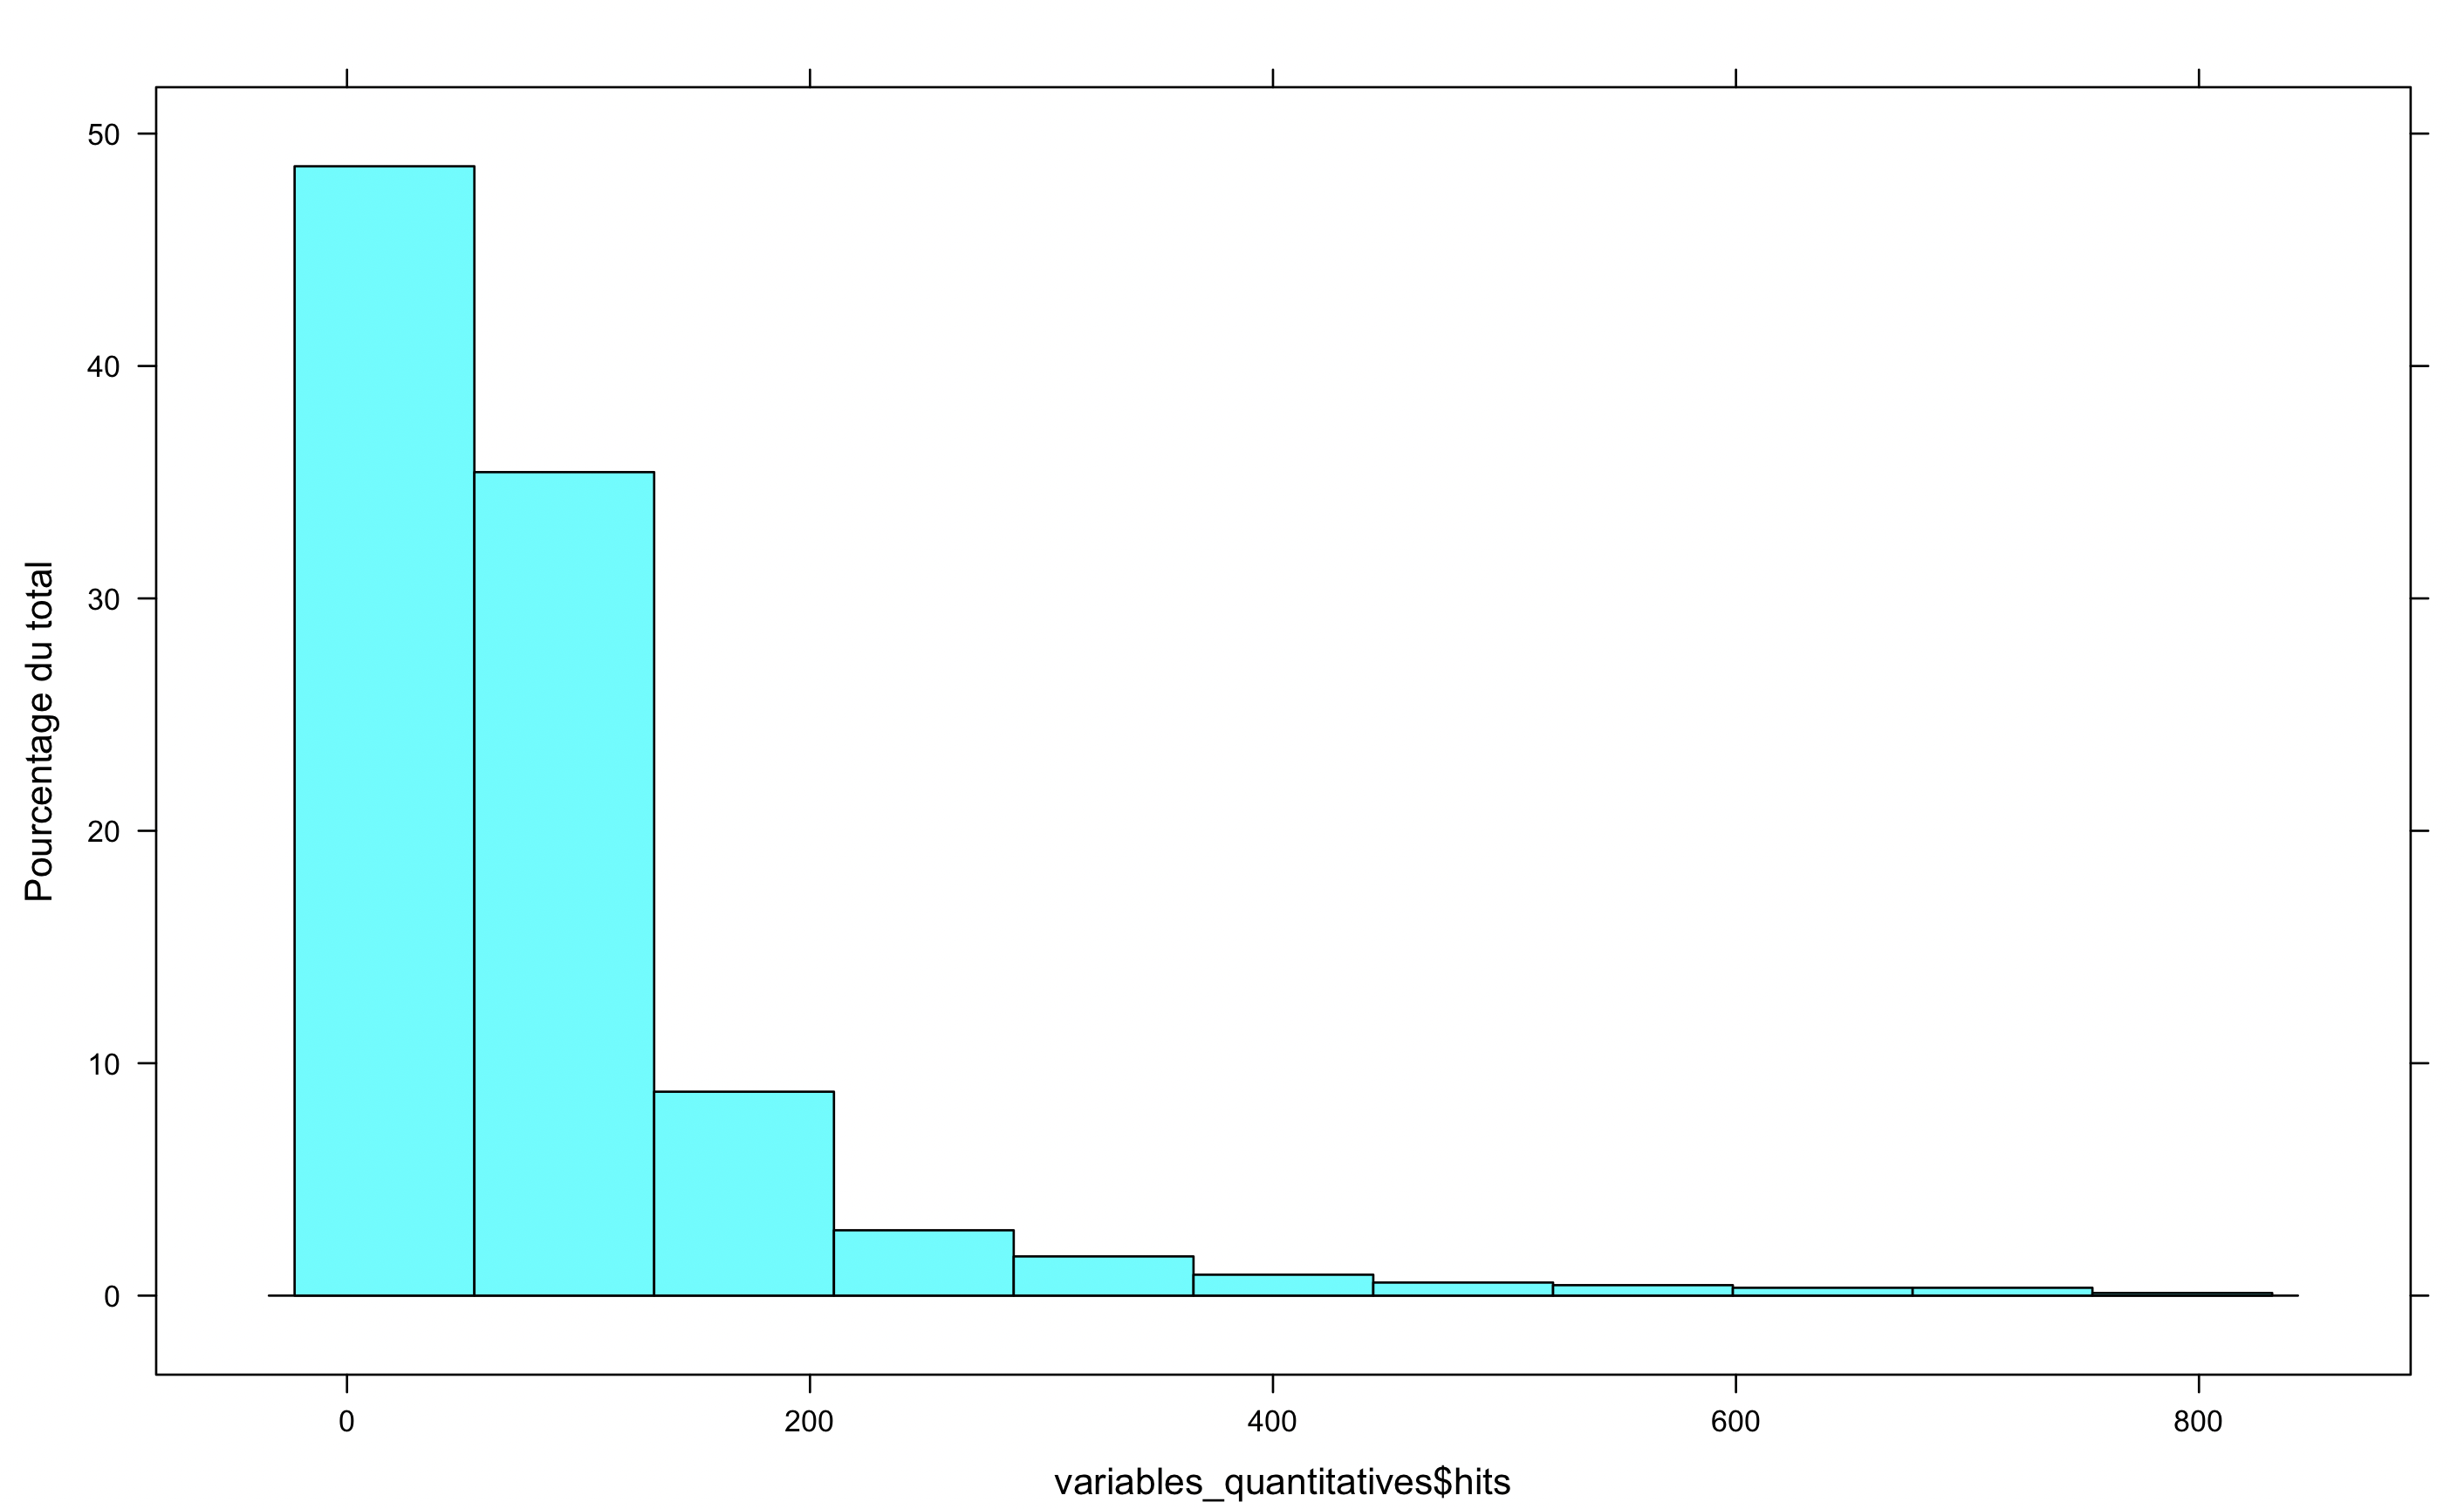
\includegraphics[width=0.45\textwidth]{scriptsR/imgs/univarie/hits_percent.png}
    }
    \hfill
    \subfloat[NewVisit: Le 70 \% des transactions ont été réalisées par des nouveaux utilisateurs.]{
        \label{new_visit}
        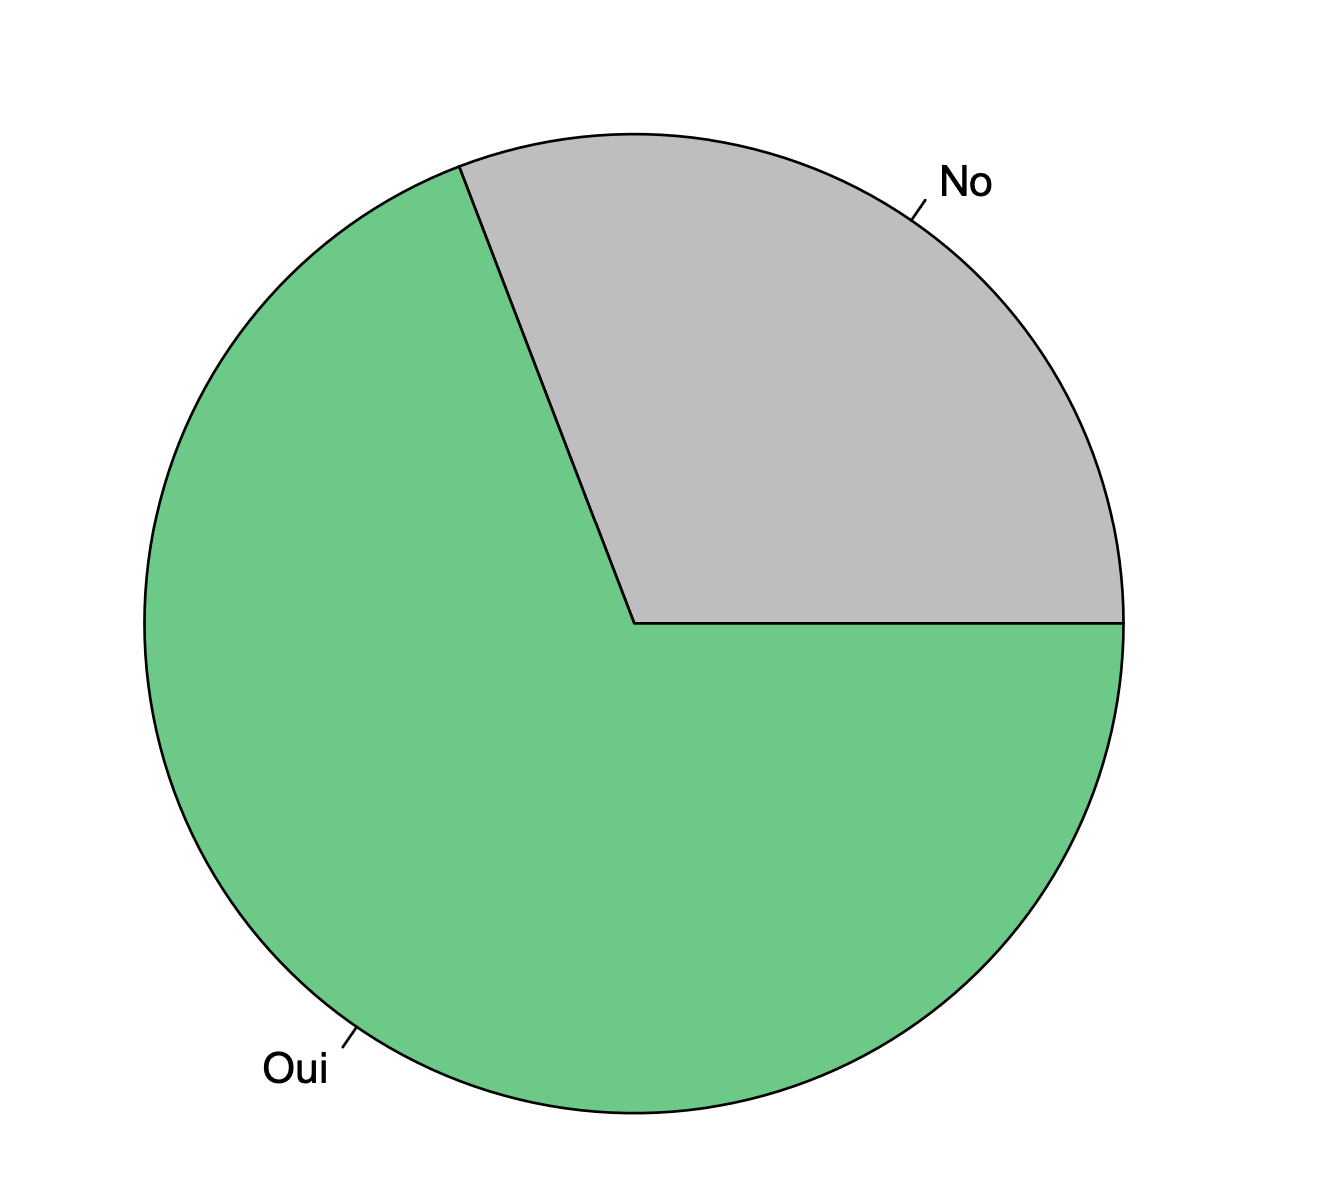
\includegraphics[width=0.45\textwidth]{scriptsR/imgs/univarie/newVisit.png}
    }
     \hfill
    \subfloat[PageViews: Pour page views, Nous avons quelques valeurs atypiques qu'on veut supprimer avant de passer a l'étape suivant. Le 80 \%  du échantillon ont entre 0 et 25 pages vues.]{
        \label{page_views}
        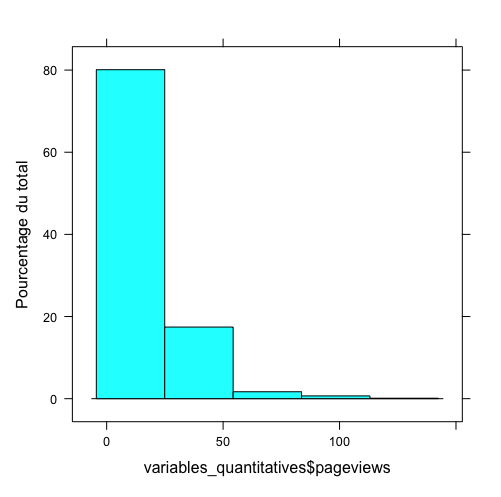
\includegraphics[width=0.45\textwidth]{scriptsR/imgs/univarie/pageviews.png}
    }
    \hfill
    \subfloat[TransactionsRevenue: La majorité de transactions sont entrées 0\euro  et  100\euro , Nous avons aussi des transactions atypiques qui  arrivent jusqu'à 800\euro ]{
        \label{transaction_revenue}
        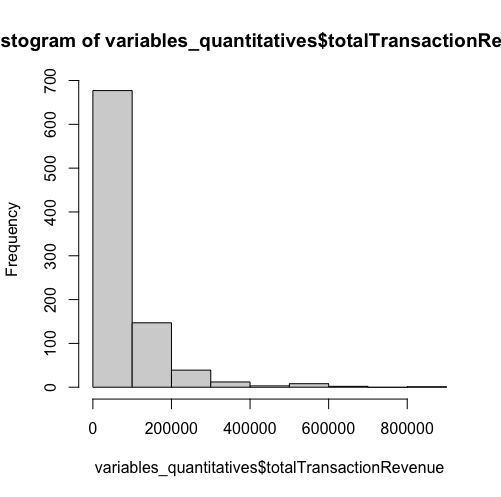
\includegraphics[width=0.45\textwidth]{scriptsR/imgs/univarie/transactionsrevenue.png}
    }
    \hfill
    \subfloat[Transactions: La majorité des individus font 1 transaction dans la session, ce qui correspond à la quantité attendu.]{
        \label{transactions}
        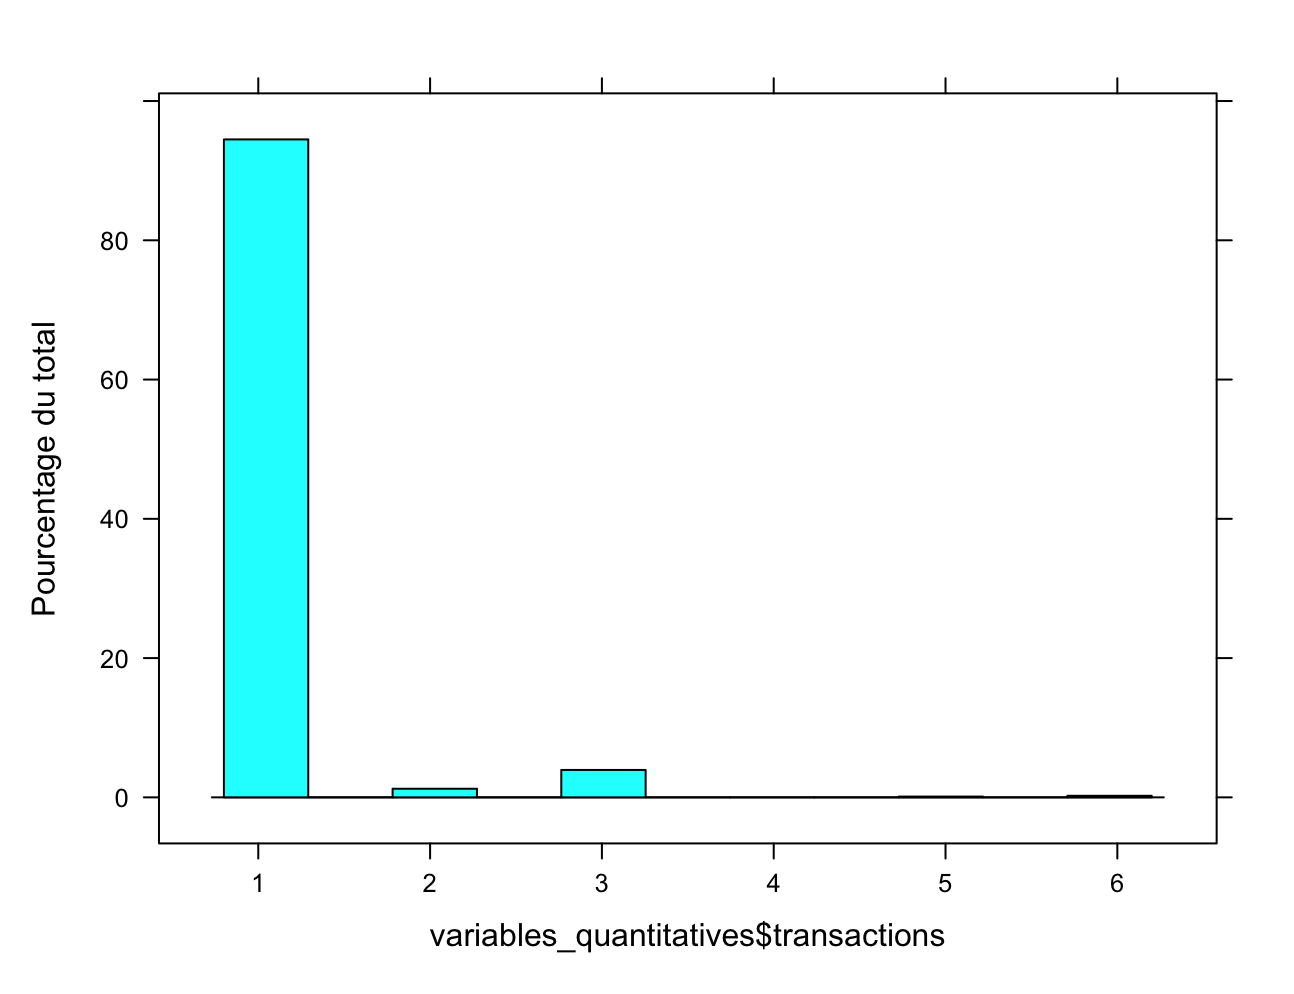
\includegraphics[width=0.45\textwidth]{scriptsR/imgs/univarie/transactionsHistogram.png}
    }
    \hfill
    \subfloat[ TimeOnSIte: Les individus prennent moins d'un minute pour effectuer au moins une transaction, le plus part entre eux, prennent moins des 20 secondes.]{
        \label{timeOnSite}
        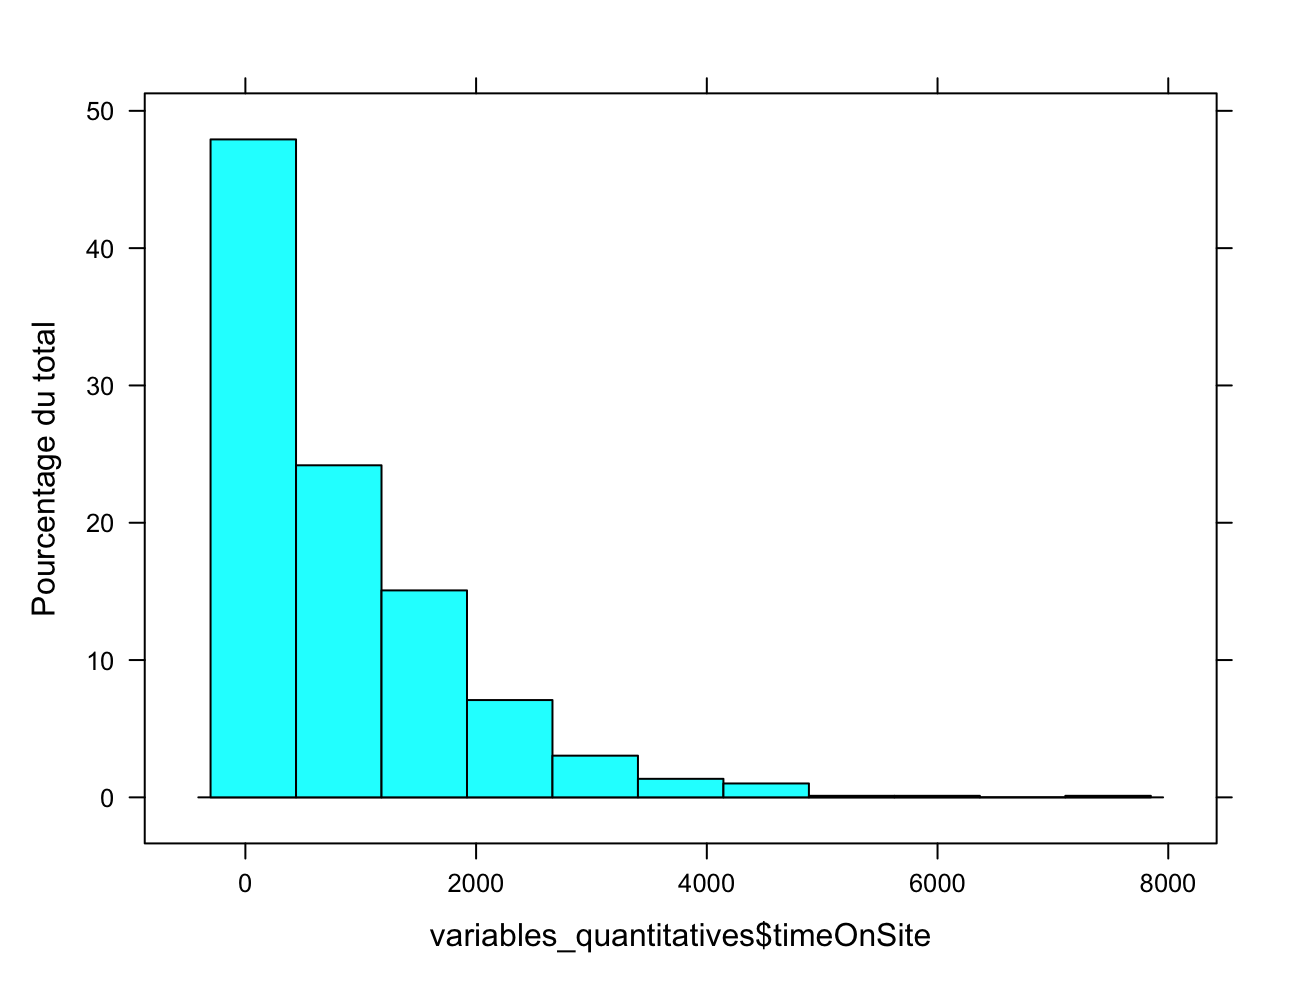
\includegraphics[width=0.45\textwidth]{scriptsR/imgs/univarie/TimeOnSIteHist.png}
    }
    \caption{Images Univariée 1}
    \label{univarie_ref}
\end{figure}


\begin{figure}[H]
\ContinuedFloat
    \centering
    \subfloat[ browserName: Chrome est le navigateur préféré des utilisateurs du échantillon suivi par safari, suivi de la version mobile de chrome.]{
        \label{browserName}
        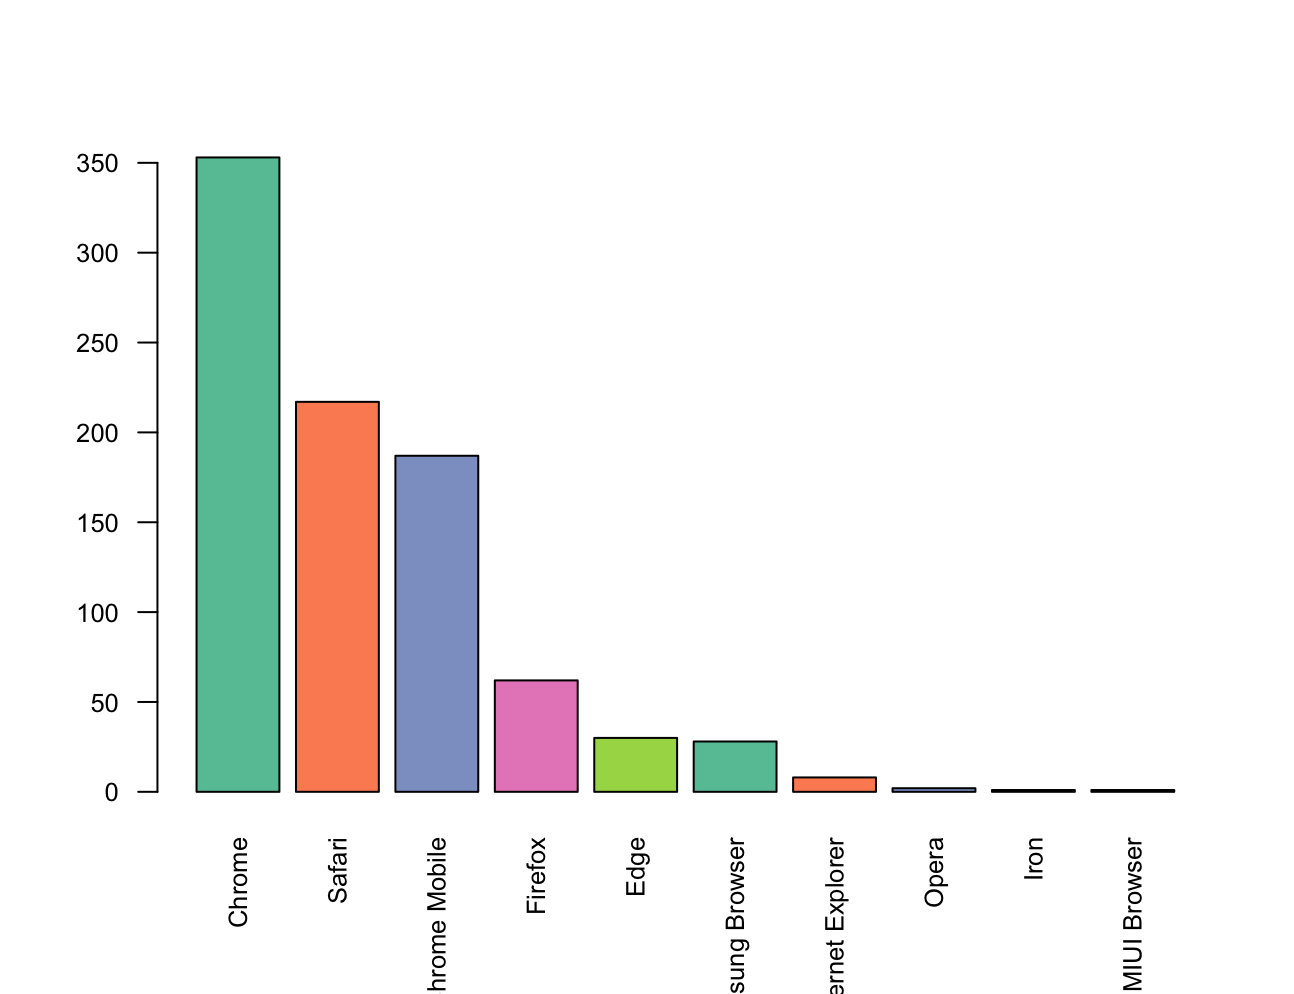
\includegraphics[width=0.45\textwidth]{scriptsR/imgs/univarie/browser_name.png}
    }
    \hfill
    \subfloat[ browserWidth: Il existe un pourcentage important d'individus qui ont effectué une transaction à partir d'un écran dont la largeur est inférieure à 500, nous pouvons en déduire qu'ils ont été réalisés depuis un appareil mobile,  suivi d'une autre plage comprise entre 1800 et 190.]{
        \label{browser_widthBoxplot}
        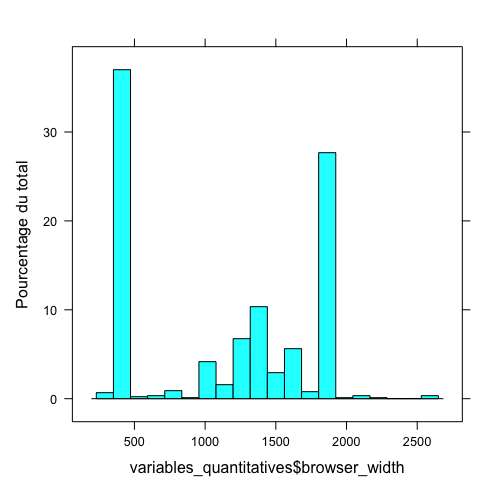
\includegraphics[width=0.45\textwidth]{scriptsR/imgs/univarie/browser_width.png}
    }
    \hfill
    \subfloat[ browserHeight: les données sont distribuées d'une manière plus uniforme, nous remarquons que les plus part de largeur d'écrans sont entre 600 pixels et 1000 pixels, nous n'observons pas de données exceptionnels ]{
        \label{browser_height_bloxplot}
        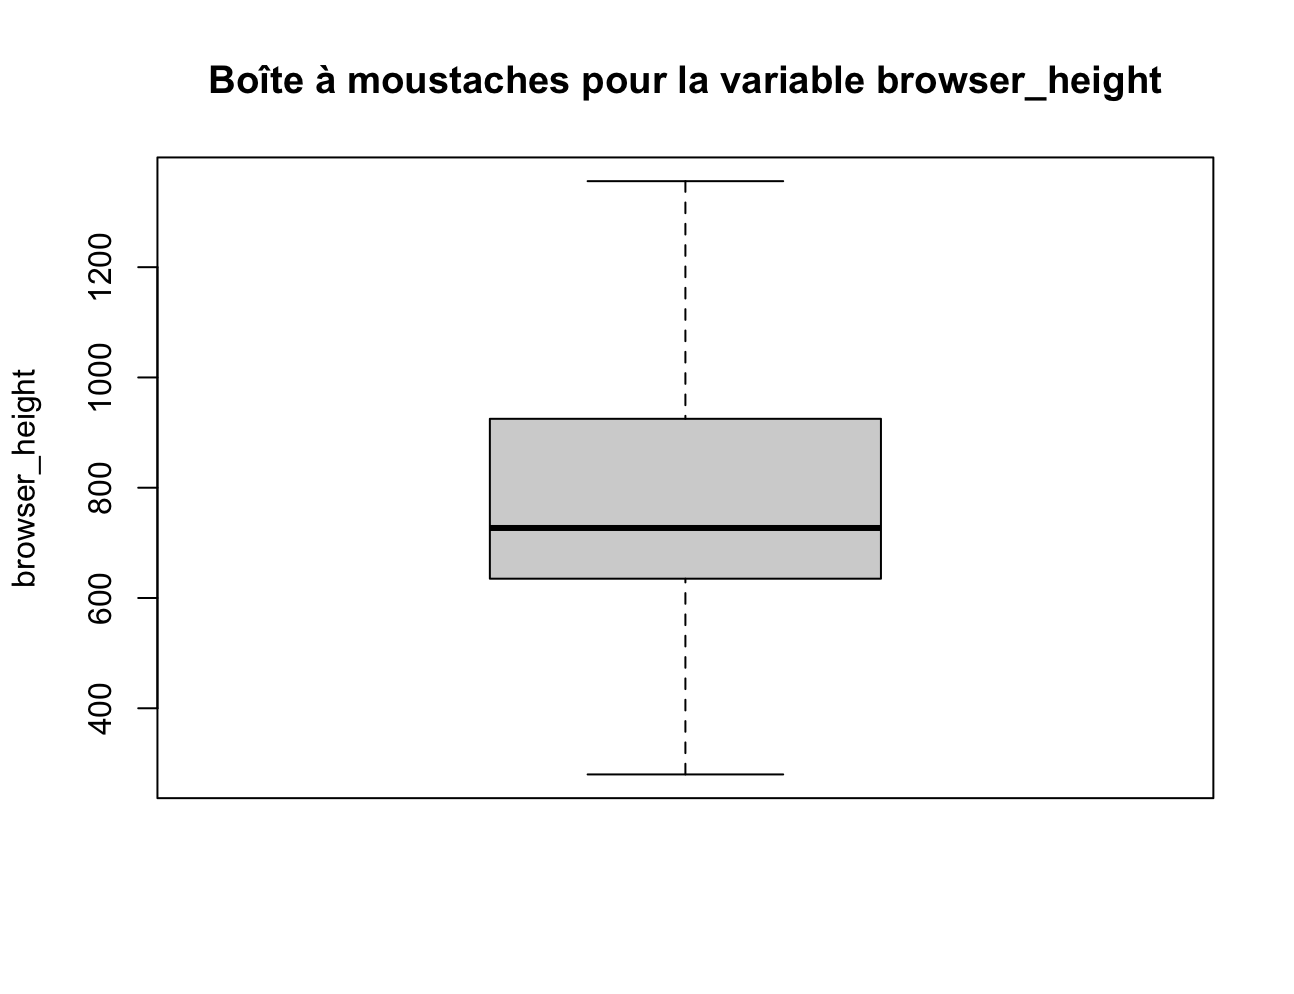
\includegraphics[width=0.45\textwidth]{scriptsR/imgs/univarie/browser_height_bloxplot.png}
    }
    \hfill
    \subfloat[deviceCategory: Contrairement a ce que nous avons constaté avec autres variables, les 57 \% des transactions ont étés réalisé depuis une laptop, suivi d'un 38\%  avec un dispositif mobile.]{
        \label{deviceCategory}
        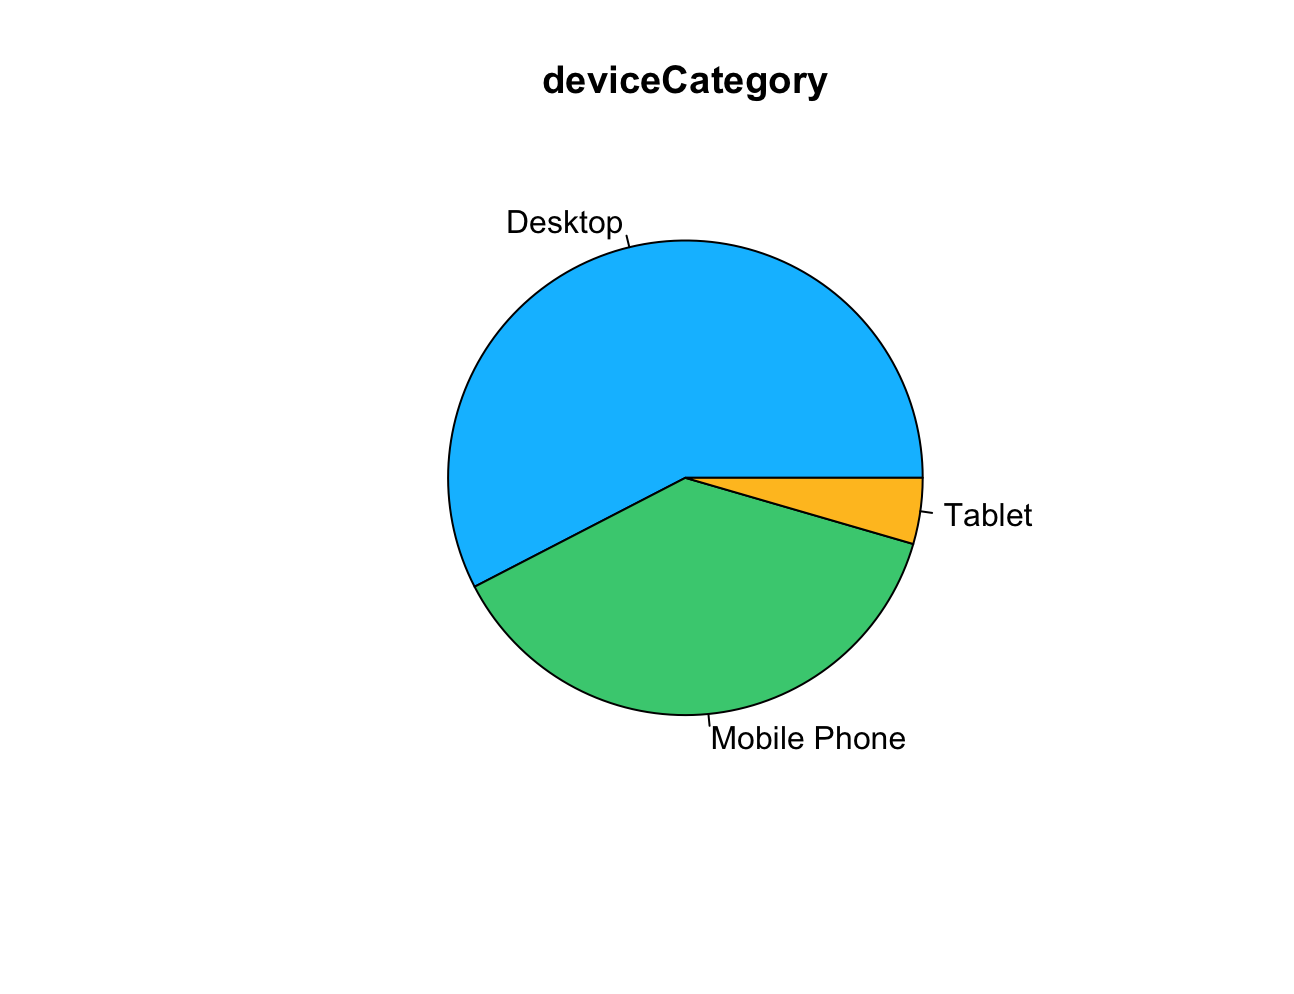
\includegraphics[width=0.45\textwidth]{scriptsR/imgs/univarie/deviceCategory.png}
    }
    \hfill
    \subfloat[operatingSys: Windows 10 est le système d'exploitation préféré du échantillon. ]{
        \label{operatingSys}
        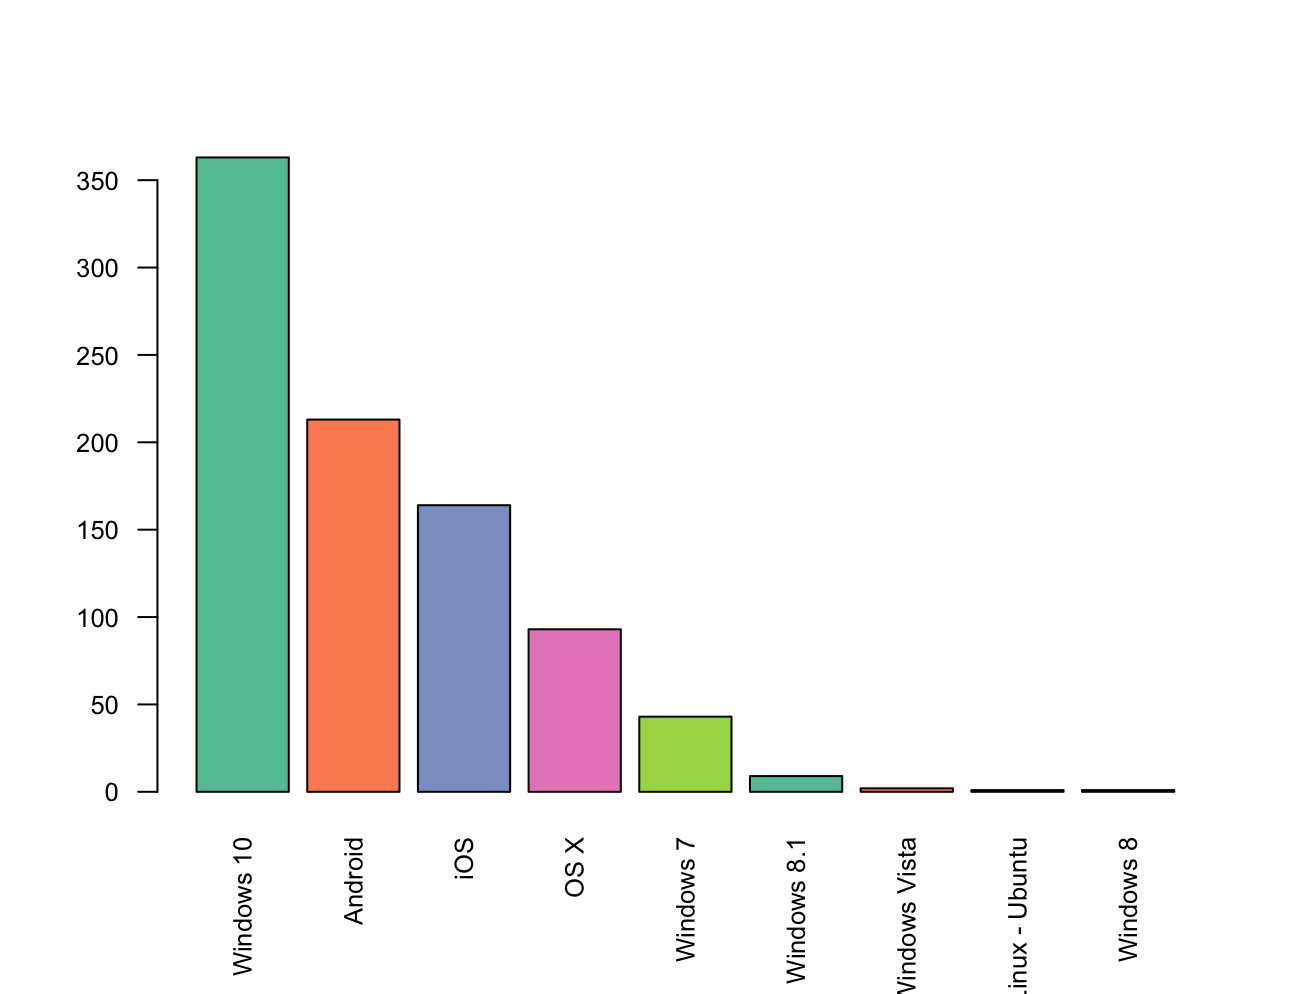
\includegraphics[width=0.45\textwidth]{scriptsR/imgs/univarie/operatingSys.png}
    }
    \hfill
    \subfloat[languageApply: L'anglais américain et le français du France sont les langues préférées des utilisateurs lorsqu'ils effectuent une transaction.]{
        \label{language}
        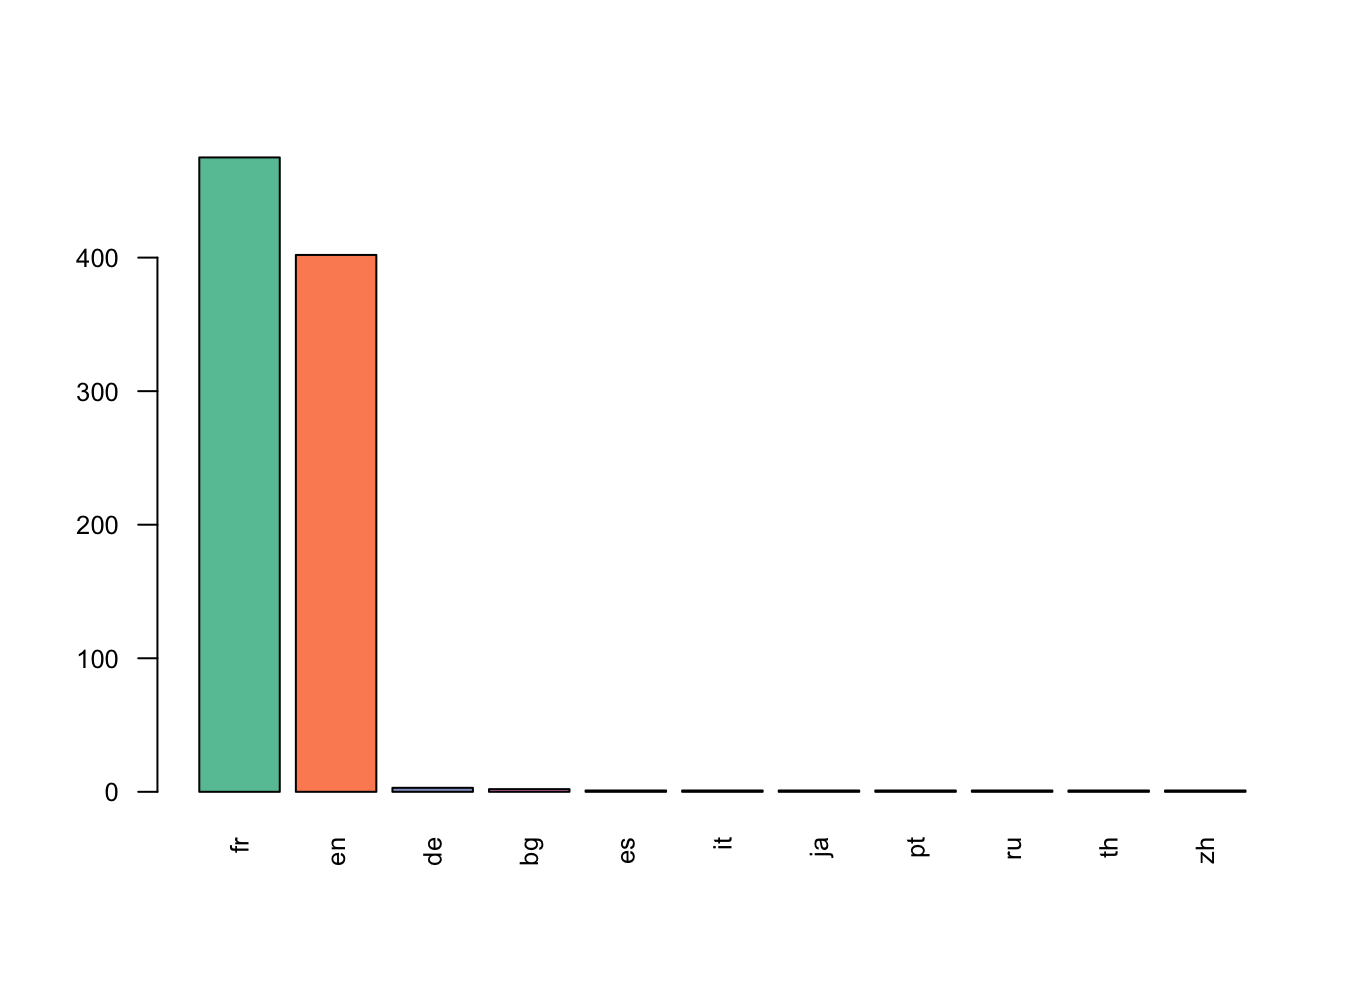
\includegraphics[width=0.45\textwidth]{scriptsR/imgs/univarie/language_apply.png}
    }
    \caption{Images Univariée 2 }
    \label{univarie_ref}
\end{figure}


\begin{figure}[H]
\ContinuedFloat
    \centering

      \subfloat[PaymentMethod: Avec plus de 600 sessions, la carte de crédit est le mode de paiement le plus utilisé pour les transats, suivi de Paypal avec un peu plus de 100 session. ]{
        \label{paymentMethod}
        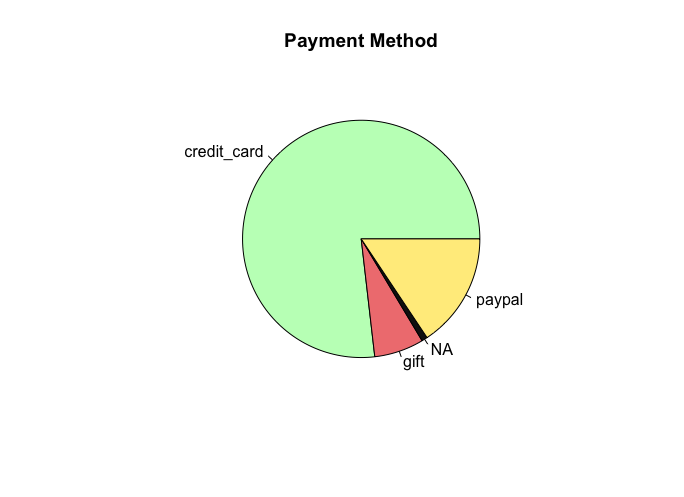
\includegraphics[width=0.45\textwidth]{scriptsR/imgs/univarie/paymentMethod.png}
    }
    \hfill
    \subfloat[itemCount: Dans un peu plus de la moitié des sessions, les transactions effectuées comprenaient 1, 2 ou 3 articles, mais un nombre important de transactions contenaient entre 5 et 10 articles. ]{
        \label{itemcountHistogram}
        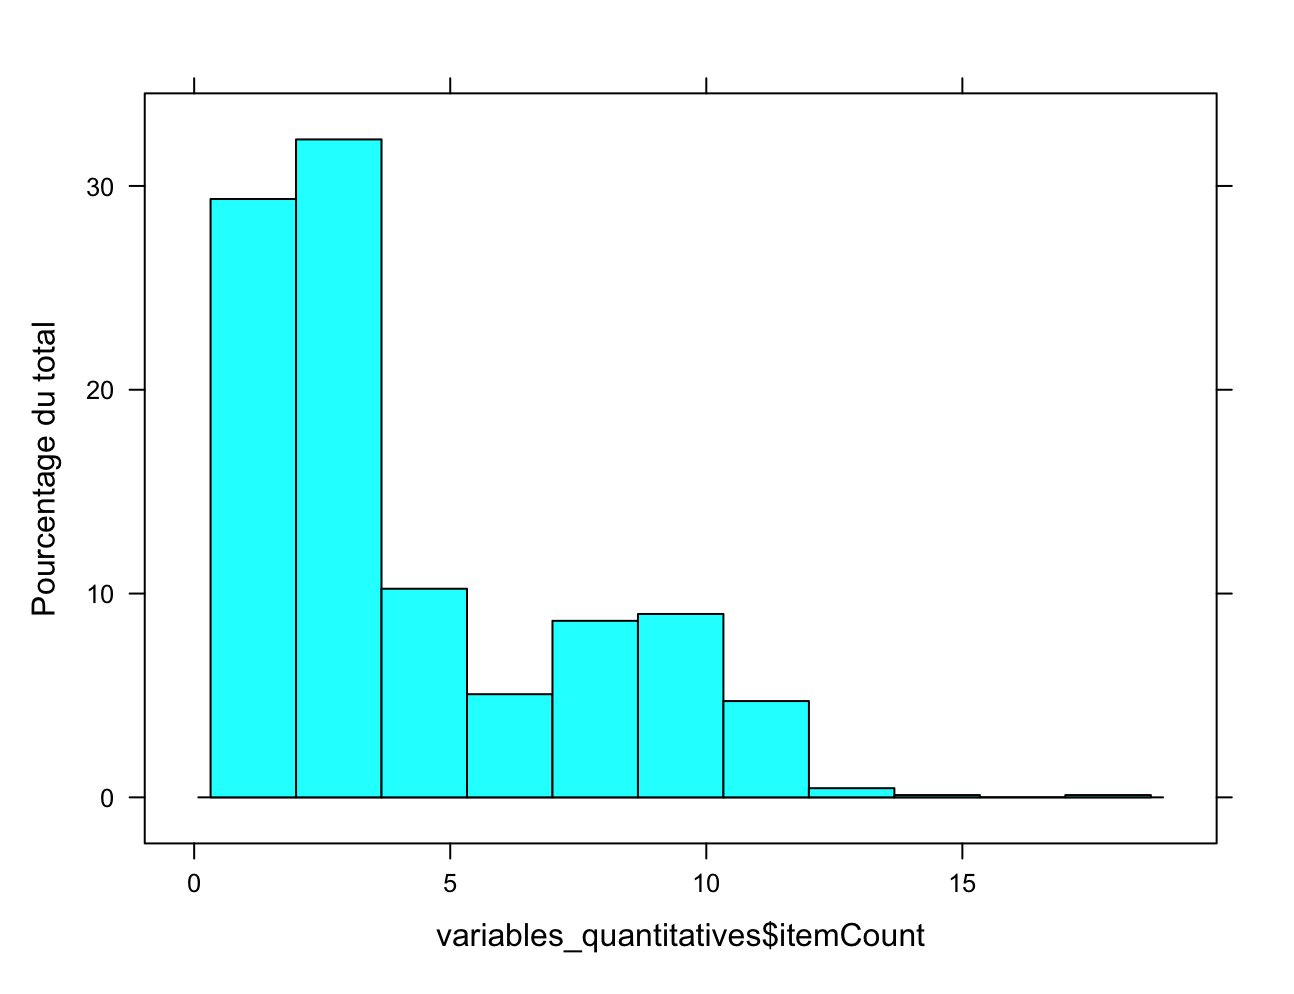
\includegraphics[width=0.45\textwidth]{scriptsR/imgs/univarie/itemcountHistogram.png}
    }
     \hfill
    \subfloat[Country: La France est le pays où se réalise plus des transactions pour ce e-commerce: 501, suivi de Netherlands avec 190. les données sont complètement cohérentes vu que c'est un e-commerce français. ]{
        \label{country}
        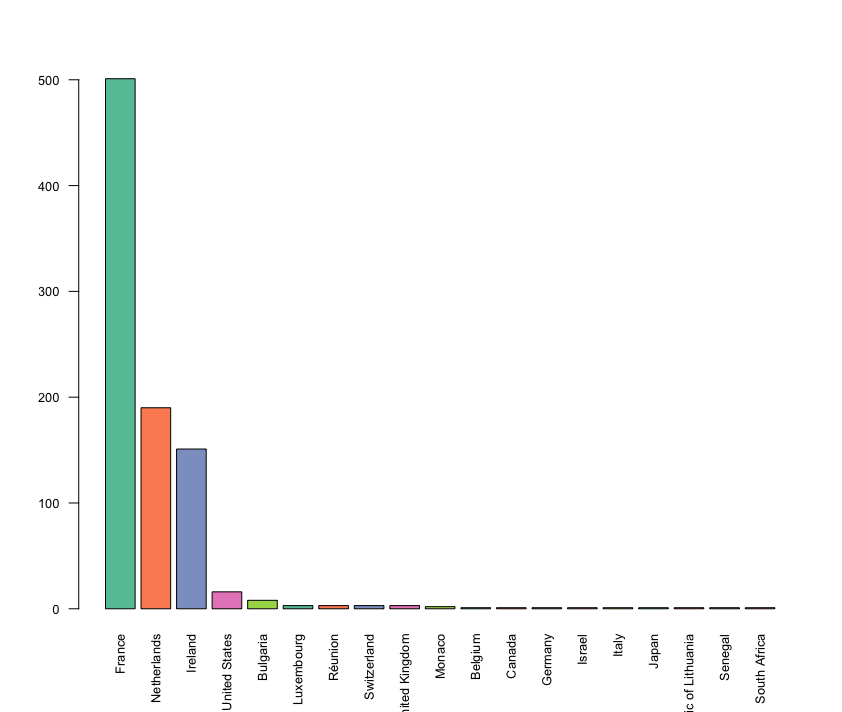
\includegraphics[width=0.45\textwidth]{scriptsR/imgs/univarie/country.png}
    }
    \hfill
    \subfloat[City: Nous avons 302 villes différentes dans l'échantillon et on a 309 transactions où on a pas des info de la ville. La ville que plus a des transactions est Paris avec 90, suivi de Dublin avec 38. ]{
        \label{cities}
        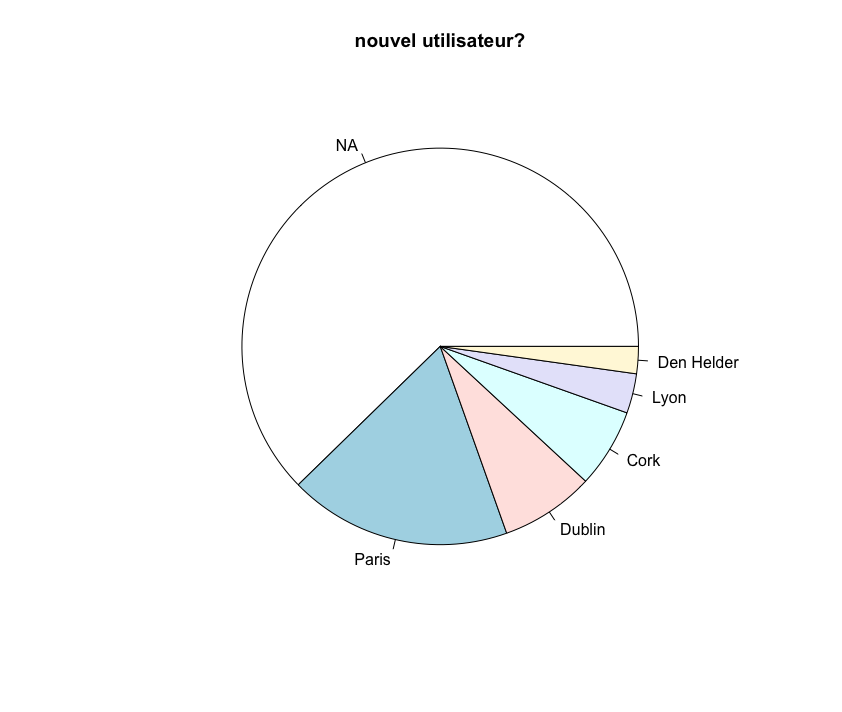
\includegraphics[width=0.45\textwidth]{scriptsR/imgs/univarie/city.png}
    }
  
    \caption{Images Univariée 3}
    \label{univarie_ref}
\end{figure}








\section{Analyse biivariée}
% !TEX root = bivariate.tex

bivariate


\section{Classification non supervisée }
% !TEX root = clasification.tex
 clasification

\section{Conclusion }
% !TEX root = conclusion.tex
 conclusion

         
\end{document}



